% The value R sits at a point in the complex plane; the path alpha (red)
% winds once around the origin while beta (blue) is a small loop. Their
% commutator alpha beta alpha^{-1} beta^{-1} keeps every phase unchanged
% yet realizes a nontrivial permutation of the roots.
% Source: book/tex/complex-ana/quintic.tex (section: Step 2, Nested Roots).
\documentclass[border=2mm]{standalone}
\usepackage{tikz}
\usetikzlibrary{arrows.meta}
\begin{document}
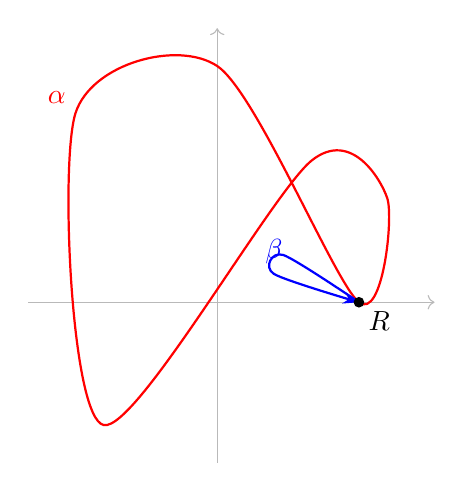
\begin{tikzpicture}[scale=1.2]
  % Complex plane axes.
  \draw[->, gray!55] (-2.0,0) -- (2.3,0);
  \draw[->, gray!55] (0,-1.7) -- (0,2.9);
  % alpha: a large loop through the origin's neighbourhood (red).
  \draw[red, thick, -{Stealth[length=2.4mm]}]
    plot[smooth cycle] coordinates
      {(1.5,0) (0,2.5) (-1.5,2) (-1.2,-1.3) (1,1.5) (1.8,1.1)};
  \node[red, above left] at (-1.5,2) {$\alpha$};
  % beta: a small loop (blue).
  \draw[blue, thick, -{Stealth[length=2mm]}]
    plot[smooth] coordinates {(1.5,0) (0.7,0.5) (0.6,0.3) (1.5,0)};
  \node[blue, above] at (0.6,0.3) {$\beta$};
  % The marked value R.
  \fill (1.5,0) circle (1.6pt) node[below right] {$R$};
\end{tikzpicture}
\end{document}
